\section{理论分析}
\label{sec:th_analysis_multiple_a_delay}

本节分析不同模型的性质。首先在 \Cref{subsec:from_mtdmdp_mdp} 中分析 \glspl{mtdmdp} 与 \glspl{mdp} 的关系。然后，在 \Cref{subsec:analysis_psmmdp_pmmmdp} 中，针对平均奖励准则，证明在 \gls{psmmdp} 或 \gls{pmmmdp} 中学习的问题等价于在底层无延迟 \gls{mdp} 中学习。最后，在 \Cref{subsec:analysis_ismmdp} 中，考虑在 \gls{ismmdp} 中学习策略的任务——这更为复杂。先说明其一些特殊性，再总结能或不能应用于此情况的 \gls{rl} 算法。读者可能注意到我们将 \gls{immmdp} 搁置了。它们确实是一种更复杂的设定，需要未来单独分析。


\subsection{从 MTD-MDP 回到 MDP}
\label{subsec:from_mtdmdp_mdp}

第一个结果展示了给定固定延迟策略时，上述分布之间的不同关系。首先给出 \gls{ismmdp} 和 \gls{immmdp} 的结果。

\begin{prop}[$\statespace$、$\augmentedstatespace$、$\statespace\times\actionspace$ 与 $\augmentedstatespace\times\actionspace$ 上分布之间的关系]
设 $\delayedpolicy$ 为 \gls{ismmdp} 或 \gls{immmdp} 上的策略，其在增广状态空间上诱导分布 $\delayeddiscountedstateoccupancydistribution[][\delayedpolicy]$。则前述分布 3 至 6 与 $\delayeddiscountedstateoccupancydistribution[][\delayedpolicy]$ 的关系如下。设 $s\in\statespace$、$x\in\augmentedstatespace$、$a\in\actionspace$，
\begin{align}
    &\discountedstateoccupancydistribution[][\delayedpolicy](x,a) = \discountedstateoccupancydistribution[][\delayedpolicy](x) \delayedpolicy(a\vert x),
    \label{eq:x_a_from_distrib_x}\\
    &\discountedstateoccupancydistribution[][\delayedpolicy](s) = \int_{\augmentedstatespace}  \delta_{s} (e_0^\top x) \delayeddiscountedstateoccupancydistribution[][\delayedpolicy](x)\;\de x
    \label{eq:s_from_distrib_x}\\
    &\discountedstateoccupancydistribution[][\delayedpolicy](s,a) = \int_{\augmentedstatespace}  \delta_{s} (e_1^\top x) \delta_{a} (e_1^\top x) \delayeddiscountedstateoccupancydistribution[][\delayedpolicy](x)\;\de x,
    \label{eq:s_a_from_distrib_x}
\end{align}
其中使用 $(e_i)_{[\![0,\delaymax]\!]}$ 作为 $\augmentedstatespace\times\actionspace$ 上的基。对于 $x=(s,a_1,\dots,a_\delaymax)$，设 $e_0^\top x=s$ 且 $e_i^\top x=a_i$。
\end{prop}
\begin{proof}
    \Cref{eq:x_a_from_distrib_x} 是 \gls{rl} 领域的已知结果。\Cref{eq:s_from_distrib_x} 使用了与 \cite[Lemma~3.1]{wu2017markov} 类似的思想，即对 $x$ 中包含的状态求边际分布。\Cref{eq:s_a_from_distrib_x} 由类似推理得到。
\end{proof}

显然，对于 \gls{psmmdp} 和 \gls{pmmmdp} 可证相同结果。
\begin{prop}[$\statespace$、$\orderdstatespace$、$\statespace\times\actionspace$ 与 $\orderdstatespace\times\actionspace$ 上分布之间的关系]
设 $\orderdpolicy$ 为 \gls{psmmdp} 或 \gls{pmmmdp} 上的策略，其在增广状态空间上诱导分布 $\delayeddiscountedstateoccupancydistribution[][\orderdpolicy]$。则前述分布 7 至 10 与 $\delayeddiscountedstateoccupancydistribution[][\delayedpolicy]$ 的关系如下。设 $s\in\statespace$、$\widebar x\in\orderdstatespace$、$a\in\actionspace$，
\begin{align}
    &\discountedstateoccupancydistribution[][\orderdpolicy](\widebar x,a) = \discountedstateoccupancydistribution[][\orderdpolicy](\widebar x) \orderdpolicy(a\vert \widebar x),
    \label{eq:x_a_from_distrib_x_past}\\
    &\discountedstateoccupancydistribution[][\orderdpolicy](s) = \int_{\orderdstatespace}  \delta_{s} (e_0^\top \widebar x) \delayeddiscountedstateoccupancydistribution[][\orderdpolicy](\widebar x)\;\de \widebar x
    \label{eq:s_from_distrib_x_past}\\
    &\discountedstateoccupancydistribution[][\orderdpolicy](s,a) = \int_{\orderdstatespace}  \delta_{s} (e_1^\top \widebar x) \delta_{a} (e_1^\top \widebar x) \delayeddiscountedstateoccupancydistribution[][\orderdpolicy](\widebar x)\;\de \widebar x,
    \label{eq:s_a_from_distrib_x_past}
\end{align}
其中将前述记号扩展到 $\orderdstatespace\times\actionspace$ 上的基 $(e_i)_{[\![-\delaymax+1,\delaymax]\!]}$。对于 $\widebar x=(s_{-\delaymax+1},\dots,s_{-1},s,a_1,\dots,a_\delaymax)$，设 $e_0^\top x=s$、$e_i^\top x=a_i$、$e_{-i}^\top x=s_{-i}$。
\end{prop}

延迟文献中一个反复出现的著名结果是 \gls{dmdp} 与具有增广状态的 \gls{mdp} 之间的等价性。我们证明类似结果对 \glspl{mtdmdp} 也成立。首先推导 \gls{ismmdp} 和 \gls{immmdp} 的结果。

\begin{prop}[\gls{immmdp} 的等价 \gls{mdp}]
\label{prop:equ_mdp_im_mtdmdp}
    对于 \gls{immmdp}，可以通过将状态空间增广到 $\augmentedstatespace=\statespace\times\actionspace^\delaymax$ 将问题还原回 \gls{mdp}。
\end{prop}
\begin{proof}
    设 $\delayedmarkovdecisionprocess_{\boldsymbol\lambda}$ 为一个 \gls{immmdp}。为证明该性质，定义一个状态空间为 $\augmentedstatespace=\statespace\times\actionspace^\delaymax$、动作空间为 $\actionspace$ 的 \gls{mdp} $\markovdecisionprocess$，使得为 $\delayedmarkovdecisionprocess_{\boldsymbol\lambda}$ 定义的任何历史依赖策略 $\delayedpolicy\in\delayedpolicyspace$ 在 $\markovdecisionprocess$ 上实现相同的回报。

    对于增广状态 $x\in\augmentedstatespace$（其中 $x=(s,a_1,\dots,a_{\delaymax})$）和某个动作 $a_{\delaymax+1}\in\actionspace$，定义 $\markovdecisionprocess$ 中的奖励为，
    \begin{align*}
        \augmentedrewardfunction(x,a_{\delaymax+1}) &=\sum_{g=0}^{\delaymax} \lambda_{g} \rewardfunction(s,a_{\delaymax+1-g}).
    \end{align*}
    现在定义 $\markovdecisionprocess$ 上两个增广状态 $x=(s,a_1,\dots,a_{\delaymax})$ 与 $x'=(s',a_1',\dots,a_{\delaymax}')$ 之间在动作 $a_{\delaymax+1}\in\actionspace$ 下的转移函数 $\augmentedtransitionfunction$：
    \begin{align*}
        \augmentedtransitionfunction(x'\vert x,a_{\delaymax+1}) = \left(\sum_{g=0}^{\delaymax}\lambda_g p_{g}(s'\vert s,a_{\delaymax+1-g})\right)\prod_{i=1}^{\delaymax}\delta_{a_{i+1}}(a_{i}').
    \end{align*}
    显然 $\markovdecisionprocess$ 是一个 \gls{mdp}。现在，设 $\delayedpolicy$ 是 $\delayedmarkovdecisionprocess_{\boldsymbol\lambda}$ 上的历史依赖策略。假设历史 $(s_0,a_0,\dots,s_{t-1},a_{t-1},s_t)\in(\statespace\times\actionspace)^t$\footnote{回顾 $\augmentedstatespace\times\actionspace$ 上的分布定义了 $\statespace\times\actionspace$ 上的分布。} 对 $\markovdecisionprocess$ 和 $\delayedmarkovdecisionprocess_{\boldsymbol\lambda}$ 相同。那么，$\delayedpolicy$ 选择的动作 $a_t$ 显然具有相同分布。$\delayedmarkovdecisionprocess_{\boldsymbol\lambda}$ 中的下一状态 $s_{t+1}$ 从 $\textstyle\sum_{g=0}^{\delaymax}\lambda_g p_g(\cdot\vert s_t,a_{t-g})$ 中采样，而根据构造，下一个增广状态 $x_{t+1}$ 中包含的状态也是如此，因为当前增广状态 $x_t$ 是 $(s_t,a_{t-\delay},\dots,a_{t-1})$。通过递推，对于 $t'>t$，历史具有相同概率。只需以相同方式初始化两个过程，即初始增广状态中包含的动作应与 $\delayedmarkovdecisionprocess_{\boldsymbol\lambda}$ 中前 $\delaymax$ 个动作具有相同概率。根据构造，这些轨迹上的奖励相同，因此回报也相同。证毕。
\end{proof}


\begin{prop}[\gls{ismmdp} 的等价 \gls{mdp}]
\label{prop:equ_mdp_is_mtdmdp}
    对于 \gls{ismmdp}，可以通过将状态空间增广到 $\augmentedstatespace=\statespace\times\actionspace^\delaymax$ 将问题还原回 \gls{mdp}。
\end{prop}
\begin{proof}
    只需移除转移概率对 $g$ 的依赖，即可应用相同的证明。
\end{proof}

类似地，对于 \gls{pmmmdp} 和 \gls{psmmdp} 有以下结果。

\begin{prop}[\gls{pmmmdp} 的等价 \gls{mdp}]
\label{prop:equ_mdp_pm_mtdmdp}
    对于 \gls{pmmmdp}，可以通过将状态空间增广到 $\orderdstatespace=\statespace^{\delaymax}\times\actionspace^{\delaymax}$ 将问题还原回 \gls{mdp}。
\end{prop}
\begin{proof}
    设 $\delayedmarkovdecisionprocess_{\boldsymbol\lambda}$ 为一个 \gls{pmmmdp}。如上所述，对于状态空间为 $\orderdstatespace=\statespace^{\delaymax}\times\actionspace^{\delaymax}$、动作空间为 $\actionspace$ 的 \gls{mdp} $\markovdecisionprocess$，对于增广状态 $x\in\orderdstatespace$（其中 $x=(s_{-\delaymax+1},\dots,s_{-1},s,a_1,\dots,a_\delaymax)$）和某个动作 $a_{\delaymax+1}\in\actionspace$，$\markovdecisionprocess$ 中的奖励定义为，
    \begin{align*}
        \higherorderrewardfunction(x,a_{\delaymax+1})
        &= \sum_{g=0}^{\delaymax} \lambda_{g} \rewardfunction(s_{\delaymax-g},a_{\delaymax+1-g}).
    \end{align*}
    考虑另一个增广状态 $x'=(s_{-\delaymax+1}',\dots,s_{-1}',s',a_1',\dots,a_\delaymax')\in\orderdpolicy$，则转移概率为，
    \begin{align*}
        \higherordertransitionfunction(x'\vert x,a_{\delaymax+1}) = \left(\sum_{g=0}^{\delaymax}\lambda_g p_{g}(s'\vert s_{\delaymax-g},a_{\delaymax+1-g})\right)\prod_{i=1}^{\delay}\delta_{a_{i+1}}(a_{i}').
    \end{align*}
    显然 $\markovdecisionprocess$ 是一个 \gls{mdp}，可以应用与之前相同的推理证明等价性。
\end{proof}


\begin{prop}[\gls{psmmdp} 的等价 \gls{mdp}]
\label{prop:equ_mdp_ps_mtdmdp}
    对于 \gls{psmmdp}，可以通过将状态空间增广到 $\orderdstatespace=\statespace^{\delaymax}\times\actionspace^{\delaymax}$ 将问题还原回 \gls{mdp}。
\end{prop}
\begin{proof}
    只需移除转移概率对 $g$ 的依赖，即可应用与 \gls{pmmmdp} 相同的证明。
\end{proof}


\subsection{PSM-MDP 和 PMM-MDP 的分析}
\label{subsec:analysis_psmmdp_pmmmdp}

在本小节中，我们特别分析平均奖励情况下的 \gls{psmmdp} 和 \gls{pmmmdp}。我们证明这些情况本质上等同于求解底层 \gls{mdp}。实际上，正如将看到的，在延迟过程的当前状态上应用无延迟策略将产生相同的平均状态-动作分布，因此获得相同的奖励。记 $(p^\pi)^{(k)}(s',a'\vert s,a)$ 为从状态 $s$ 出发、执行动作 $a$ 后遵循策略 $\pi$，在 $k$ 步内到达状态-动作 $(s',a')$ 的概率。首先给出 \gls{psmmdp} 的结果。

\begin{lemma}
\label{lem:same_distrib_psmmdp}
    设 $\pi$ 为 \gls{mdp} $\markovdecisionprocess$ 中的策略，满足 $\textstyle\lim_{k\rightarrow\infty}(p^\pi)^{(k)}(s,a\vert s',a')= \averagestateoccupancydistribution(s,a)$。
    则对于基于 $\markovdecisionprocess$ 构建的 \gls{psmmdp} $\delayedmarkovdecisionprocess$，将 $\pi$ 应用于其当前状态在 $\statespace\times\actionspace$ 上产生与 $\markovdecisionprocess$ 中相同的平均状态-动作占用分布 $\averagestateoccupancydistribution$。
\end{lemma}
\begin{proof}
    固定策略 $\pi$ 后，底层 \gls{mdp} 变为 \gls{mc}。将此结果 \cite[Theorem~2.1]{adke1988limit} 应用于该马尔可夫链，可得对于 $(s',a')\in\statespace\times\actionspace$，
    \begin{align*}
        \lim_{k\rightarrow\infty}(\higherordertransitionfunction^\pi)^{(k)}(s',a' \vert x) = \averagestateoccupancydistribution(s,a),
    \end{align*}
    其中 $x=(s,a_1,\dots,a_\delay)\in\augmentedstatespace$，且
    \begin{align*}
        (\higherordertransitionfunction^\pi)^{(1)}(s',a' \vert x)= \left(\sum_{g=1}^{\delaymax} \lambda_g \transitionfunction(s_t\vert s,a_{\delaymax+1-g}) + \lambda_g \transitionfunction(s\vert s,a')\right)\pi(a'\vert s).
    \end{align*}
    上式中括号内的项正是 \gls{psmmdp} 转移函数的定义。证毕。
\end{proof}

由上述结果显然可得以下定理。
\begin{thm}
\label{th:psmmdp_same}
    设 $\pi$ 为 \gls{mdp} $\markovdecisionprocess$ 中的策略，满足 $\lim_{k\rightarrow\infty}(p^\pi)^{(k)}(s,a\vert s',a')= \discountedstateoccupancydistribution[][\pi](s,a)$，且 $\delayedmarkovdecisionprocess_{\boldsymbol{\lambda}}$ 为基于 $\markovdecisionprocess$ 构建的 \gls{psmmdp}。
    则将该策略 $\pi$ 应用于 \gls{psmmdp} 的当前状态所获得的平均奖励与其在 $\markovdecisionprocess$ 中相同。
\end{thm}
\begin{proof}
    根据 \Cref{lem:same_distrib_psmmdp}，$\pi$ 在 $\delayedmarkovdecisionprocess_{\boldsymbol{\lambda}}$ 和 $\markovdecisionprocess$ 中的 $\statespace\times\actionspace$ 上具有相同分布。根据 \gls{psmmdp} 中延迟的定义，$\pi$ 在两个过程中也具有相同的平均奖励。
\end{proof}

现在将注意力转向 \gls{pmmmdp}。假设 \gls{mtdmdp} 模型的转移函数是齐次的，即对于 $s,s'\in\statespace$ 和 $a\in\actionspace$：
\begin{align*}
    \transitionfunction_g(s'\vert s,a)=\transitionfunction^{(g+1)}(s'\vert s,a).
\end{align*}
这样，\Cref{def:pmmmdp} 中定义的 \gls{pmmmdp} 转移变为，
\begin{align*}
    \probability(S_{t+1}=s_{t+1}\vert& S_{t}=s_{t},A_{t}=a_{t},\dots,S_{t-\delaymax}=s_{t-\delaymax},A_{t-\delay}=a_{t-\delaymax})
    \\
    &= \sum_{g=0}^\delaymax \lambda_g \transitionfunction^{(g+1)}(s_{t+1}\vert s_{t-g},a_{t-g}).
\end{align*}

在此假设下，可以证明以下结果。
\begin{lemma}
\label{lem:same_distrib_pmmmdp}
    设 $\pi$ 为 \gls{mdp} $\markovdecisionprocess$ 中的策略，满足 $\textstyle\lim_{k\rightarrow\infty}(p^\pi)^{(k)}(s,a\vert s',a')= \averagestateoccupancydistribution(s,a)$。
    则对于基于 $\markovdecisionprocess$ 构建的齐次 \gls{pmmmdp} $\delayedmarkovdecisionprocess$，将 $\pi$ 应用于其当前状态在 $\statespace\times\actionspace$ 上产生与 $\markovdecisionprocess$ 中相同的平均状态-动作占用分布 $\averagestateoccupancydistribution$。
\end{lemma}
\begin{proof}
    如前所述，固定策略 $\pi$ 后，底层 \gls{mdp} 变为 \gls{mc}。将此结果 \cite[Proposition~4]{berchtold1996modelisation} 应用于该马尔可夫链，可得对于 $(s',a')\in\statespace\times\actionspace$，
    \begin{align*}
        \lim_{k\rightarrow\infty}(\higherordertransitionfunction^\pi)^{(k)}(s',a' \vert x) = \averagestateoccupancydistribution(s,a),
    \end{align*}
    其中 $x=(s,a_1,\dots,a_\delay)\in\augmentedstatespace$，且
    \begin{align*}
        (\higherordertransitionfunction^\pi)^{(1)}(s',a' \vert x)= \left(\sum_{g=1}^{\delaymax} \lambda_g \transitionfunction^{(g)}(s_t\vert s,a_{\delaymax+1-g}) + \lambda_g \transitionfunction(s\vert s,a')\right)\pi(a'\vert s).
    \end{align*}
    上式中括号内的项正是齐次 \gls{pmmmdp} 转移函数的定义。证毕。
\end{proof}
然后，采用与 \gls{psmmdp} 相同的证明，得到以下结果。
\begin{thm}
\label{th:pmmmdp_same}
    设 $\pi$ 为 \gls{mdp} $\markovdecisionprocess$ 中的策略，满足 $\lim_{k\rightarrow\infty}(p^\pi)^{(k)}(s,a\vert s',a')= \discountedstateoccupancydistribution[][\pi](s,a)$，且 $\delayedmarkovdecisionprocess_{\boldsymbol{\lambda}}$ 为基于 $\markovdecisionprocess$ 构建的齐次 \gls{pmmmdp}。
    则将该策略 $\pi$ 应用于 \gls{pmmmdp} 的当前状态所获得的平均奖励与其在 $\markovdecisionprocess$ 中相同。
\end{thm}


\subsection{ISM-MDP 的分析}
\label{subsec:analysis_ismmdp}
现在将更详细地分析 \gls{ismmdp} 的情况，从延迟 \gls{rl} 的角度看，这或许更有趣。诚然，如前所述，\glspl{ismmdp} 将前几章研究的常值延迟作为特例包含在内。由于希望研究延迟向量 $\boldsymbol\lambda$ 的影响，记 $\expectedreturn[\gamma][\delayedpolicy](\boldsymbol\lambda)$ 为延迟策略 $\delayedpolicy$ 在 $\boldsymbol\lambda$-延迟 \gls{ismmdp} 中的期望 $\gamma$ 折扣回报，$\averagereturnfunction[\delayedpolicy](\boldsymbol\lambda)$ 为其平均奖励。

如 \Cref{th:perf_delay_vector_all_weight} 所示，较高延迟分配的权重越多，性能越低，这似乎是合理的。回顾由于 \glspl{ismmdp} 将常值 \glspl{dmdp} 作为特例包含，\Cref{th:perf_delay_vector_all_weight} 可应用于权重全部集中在单个索引上的延迟向量。现在感兴趣的是研究更一般的结果，其中延迟向量 $\boldsymbol\lambda$ 的权重分布在不同的值上。首先展示一个可能反直觉的结果。

推测延迟均值越高则性能越低似乎是合理的。然而，我们通过 \Cref{fig:counter_example_mtmdp} 的反例证明这是错误的。在此 \gls{mdp} 中考虑两个智能体。第一个智能体（智能体 1）的延迟权重为 $\lambda_0=\epsilon, \lambda_1=0,\lambda_2=1-\epsilon$，而第二个智能体（智能体 2）的所有权重在 $\lambda_1$ 上，即 $\lambda_0=\lambda_2=0$。对于 $\epsilon<0.5$，智能体 1 承受的延迟比智能体 2 更大。然而，在此 \gls{mdp} 中，智能体的动作对转移没有影响，因此智能体 1 可以优化其一步奖励，而智能体 2 不能。智能体 1 的最优策略是 $\pi(s_1)=b$ 和 $\pi(s_0)=a$，产生的一步期望奖励为 $1 \cdot\epsilon+ 0.5\cdot(1-\epsilon)=0.5( 1+\epsilon)$。相反地，智能体 2 的一步期望奖励为 $0.5$。
\begin{figure}[t]
    \centering
    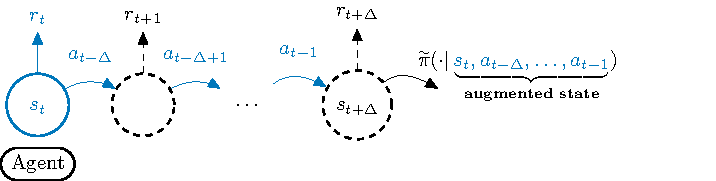
\includegraphics[bylabel=counterexamplemtmdp]{img/thesis_plots.pdf}
    \caption{针对"平均延迟越高则性能越低"这一推测的反例。
    智能体在两个状态中各有两个动作 $a$ 和 $b$。无论采取什么动作、处于什么状态，智能体都有 $1/2$ 的概率转移到另一个状态，$1/2$ 的概率保持在当前状态。奖励为 $r(s_1,b)=r(s_0,a)=1$ 和 $r(s_0,b)=r(s_1,a)=0$。奖励和转移函数经过特殊定义，使得两个智能体中，期望延迟较小但无延迟权重 $\lambda_0$ 上质量较小的那个表现更差。}
    \label{fig:counter_example_mtmdp}
\end{figure}

因此，需要找到另一种比较两个延迟向量的方法。将 $\boldsymbol\lambda$ 的分布作为整体来考虑的一种方式是考虑其累积分布。这是以下猜想的内容。

\begin{conj}
\label{conj:delay_cumulativ_distrib}
    设 $\boldsymbol\lambda$ 和 $\boldsymbol\lambda'$ 为两个延迟向量。记 $F_{\boldsymbol\lambda}$ 和 $F_{\boldsymbol\lambda}'$ 分别为其累积分布，如 \Cref{fig:hist_delay} 所示。如果对于任意 $i\in\naturalnumbers$：
    \begin{align*}
        F_{\boldsymbol\lambda}(i) \ge F_{\boldsymbol\lambda}'(i),
    \end{align*}
    则它们的最优期望折扣回报和平均奖励满足，
    \begin{align*}
        &\expectedreturn[\gamma][\star](\boldsymbol\lambda) \ge \expectedreturn[\gamma][\star](\boldsymbol\lambda')
        \\
        &\averagereturnfunction[\star](\boldsymbol\lambda)\ge\averagereturnfunction[\star](\boldsymbol\lambda').
    \end{align*}
\end{conj}

\begin{figure}[t]
    \centering
    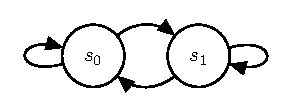
\includegraphics[labelmtd=histogramdelayvector]{img/thesis_plots_mtd.pdf}
    \caption{延迟向量 $\boldsymbol\lambda$ 示例及其累积分布函数。权重 $\lambda_i$ 对应于延迟 $i$。}
    \label{fig:hist_delay}
\end{figure}

作为该猜想的论据，我们提供以下思路。设 $\delayedmarkovdecisionprocess$ 和 $\delayedmarkovdecisionprocess'$ 是两个 \glspl{ismmdp}，其延迟向量分别为 $\boldsymbol\lambda$ 和 $\boldsymbol\lambda'$。假设 $\forall i\in\naturalnumbers, F_{\boldsymbol\lambda}(i) \ge F_{\boldsymbol\lambda}'(i)$ 且 $\boldsymbol\lambda$ 的所有权重集中在 $\lambda_\delay$（其中 $\delay\in[\![0,\delaymax]\!]$）。对于策略 $\delayedpolicy'$、增广状态 $x_t=(s_t,a_{t-\delaymax},\dots,a_{t-1})$ 和动作 $a_{t}\sim\delayedpolicy'$，在 $\delayedmarkovdecisionprocess'$ 中底层 \gls{mdp} 的新状态按以下分布采样：
\begin{align}
    s_{t+1}\sim p(\cdot\vert x_t,a_{t})= \sum_{g=\delay}^{\delaymax'}\lambda_g' \transitionfunction(\cdot\vert s_t,a_{t-g}).\label{eq:proba_trans_plus_delayed}
\end{align}
注意求和从 $\delay$ 开始，因为 $\forall i\in\naturalnumbers, F_{\boldsymbol\lambda}(i) \ge F_{\boldsymbol\lambda}'(i)$ 且 $\boldsymbol\lambda$ 的所有权重在 $\lambda_\delay$ 上。在 $\delayedmarkovdecisionprocess$ 中，智能体在时刻 $t$ 选择的动作将在时刻 $t+\delay$ 精确执行。因此可以在 $\delayedmarkovdecisionprocess$ 中构建策略 $\delayedpolicy$，使其在时刻 $t-\delay$ 选择的动作精确复现 \Cref{eq:proba_trans_plus_delayed} 的概率。形式上，这种情况发生在：
\begin{align*}
    \delayedpolicy(a\vert x_{t-\delay}) = \sum_{g=\delay}^{\delaymax'}\lambda_g'  \delta_{a_{t-g}}(a).
\end{align*}
因此，该智能体将以不同于 $\delayedpolicy'$ 的分布来为其增广状态填充动作。然而，如果 $\delayedpolicy$ 是基于历史的，它可以保留 $\delayedpolicy'$ 缓冲区中应有的动作记忆。但技术复杂性在于过程的初始化。如果 $\delayedmarkovdecisionprocess$ 和 $\delayedmarkovdecisionprocess'$ 以其缓冲区中相同的动作序列开始，由于延迟向量不同，$\statespace$ 中的第一个状态将从不同的分布中采样，而智能体对此无法控制。

接下来，通过评估延迟对方差的影响来继续研究延迟的影响。我们证明不仅性能随延迟增加而下降，而且期望回报或平均奖励的方差也在缩小。该结果适用于常值延迟 \gls{dmdp}。

\begin{prop}
\label{pp:var_ismmdp}
    设 $\delayedmarkovdecisionprocess_{1}$ 和 $\delayedmarkovdecisionprocess_{2}$ 为两个一致的 \glspl{dmdp}，其常值延迟分别为 $\delay_1$ 和 $\delay_2$，增广状态空间分别为 $\augmentedstatespace_1$ 和 $\augmentedstatespace_2$。假设 $\delay_1<\delay_2$。考虑 $\delayedpolicy_2$ 为 $\delayedmarkovdecisionprocess_{2}$ 上具有 $\sigma$-有限占用测度的策略。则存在 $\delayedmarkovdecisionprocess_{1}$ 上的策略 $\delayedpolicy_1$，使得 $\forall x_1\in\augmentedstatespace_1$ 有 $\mathbb{E}^{\delayedpolicy_1}[Y\vert x_1]=\mathbb{E}^{\delayedpolicy_2}[Y\vert x_1]$，且
    \begin{align*}
        \mathbb{V}\mathrm{ar}^{\delayedpolicy_2}\left[\mathbb{E}^{\delayedpolicy_2}[Y\vert a,x_2]\right]\le\mathbb{V}\mathrm{ar}^{\delayedpolicy_1}\left[\mathbb{E}^{\delayedpolicy_1}[Y\vert a,x_1]\right],
    \end{align*}
    其中 $x_2\in\augmentedstatespace_2$ 是从 $x_1$ 构建的增广状态，$Y$ 表示无限时域期望折扣回报或平均奖励的随机变量。项 $\mathbb{E}^{\pi}[Y\vert a,x]$ 为策略 $\pi$ 下从增广状态 $x$ 出发并首先选择动作 $a$ 时 $Y$ 的条件期望，而 $\mathbb{V}\mathrm{ar}^{\pi}$ 表示策略 $\pi$ 诱导的状态-动作分布下的方差。
\end{prop}
\begin{proof}
    回顾全方差公式；对于随机变量 $X$ 和 $Y$（$Y$ 具有有限方差），有
    \begin{align*}
        \variance[Y] = \expectedvalue\left[\variance[Y\vert X]\right] + \variance\left[\expectedvalue[Y\vert X]\right].
    \end{align*}
    将此结果应用于期望回报情况下的 $\textstyle Y=\sum_{t=0}^\infty \gamma^{t} r(s_{t},a_{t})$ 或平均奖励情况下的 $\textstyle Y=\frac{1}{H}\sum_{t=0}^\infty r(s_{t},a_{t})$\footnote{由于两种情况的证明类似，我们在记号上不做区分。}。注意，根据奖励有界的假设（$0\le r(s,a)\le \maximumreward$），$Y$ 具有有限方差。现在，设 $\delayedpolicy_2$ 为 $\delayedmarkovdecisionprocess_{2}$ 中具有 $\sigma$-有限占用测度的策略。根据 \Cref{corol:markov_optimal_delayed_equiv}，$\delayedmarkovdecisionprocess_{1}$ 中存在一个马尔可夫策略，其在 $\augmentedstatespace_1\times\actionspace$ 上的状态占用测度与 $\delayedpolicy_2$ 相同。根据 \cite[Lemma~1]{laroche2022non}，它们具有相同的期望回报或平均奖励。这表明 $\mathbb{E}^{\delayedpolicy_1}[Y]=\mathbb{E}^{\delayedpolicy_2}[Y]$，特别地，对于动作 $a\in\actionspace$ 和增广状态 $x_2\in\augmentedstatespace_2$，有 $\mathbb{E}^{\delayedpolicy_1}[Y\vert a,x_2]=\mathbb{E}^{\delayedpolicy_2}[Y\vert a,x_2]$。现在回顾，给定两个随机变量 $X_1$ 和 $X_2$，有
    \begin{align*}
        \variance\left[\expectedvalue[Y\vert X_1]\right]\le \variance\left[\expectedvalue[Y\vert X_1,X_2]\right].
    \end{align*}
    因此，如果也将 $x_1\in\augmentedstatespace_1$ 记为 $\delayedmarkovdecisionprocess_1$ 中的当前增广状态，则有
    \begin{align*}
        \mathbb{V}\mathrm{ar}^{\delayedpolicy_2}\left[\mathbb{E}^{\delayedpolicy_2}[Y\vert a,x_2]\right] &\le \mathbb{V}\mathrm{ar}^{\delayedpolicy_2}\left[\mathbb{E}^{\delayedpolicy_2}[Y\vert a,x_2,x_1]\right]
        \\
        &=\mathbb{V}\mathrm{ar}^{\delayedpolicy_2}\left[\mathbb{E}^{\delayedpolicy_2}[Y\vert a,x_1]\right],
    \end{align*}
    其中注意 $Y$ 仅依赖于未来奖励，且 $x_1$ 包含比 $x_2$ 更新的信息，因为 $\delay_1<\delay_2$。最后一个等式基于底层过程的马尔可夫性成立。接下来，将上述方程的最后一项在 $\delayedpolicy_1$ 诱导的分布下表达：
    \begin{align}
        \mathbb{V}\mathrm{ar}^{\delayedpolicy_2}\left[\mathbb{E}^{\delayedpolicy_2}[Y\vert a,x_1]\right]
        &= \mathbb{V}\mathrm{ar}^{\delayedpolicy_2}\left[\mathbb{E}^{\delayedpolicy_1}[Y\vert a,x_1]\right]\label{eq:same_return_f}
        \\
        &= \mathbb{V}\mathrm{ar}^{\delayedpolicy_1}\left[\mathbb{E}^{\delayedpolicy_1}[Y\vert a,x_1]\right]\label{eq:same_distrib_f},
    \end{align}
    其中 \Cref{eq:same_return_f} 成立是因为策略具有相同回报，\Cref{eq:same_distrib_f} 成立是因为策略在 $\augmentedstatespace_1\times\actionspace$ 上具有相同的状态占用测度。合并这两个方程即得结果。
\end{proof}

该结果表明，延迟越高，智能体的控制越弱，其回报的方差越小。延迟策略可获得回报的范围随延迟增加而缩小。在极限情况下，当延迟趋于无穷时，智能体不再控制动作序列，期望回报或平均奖励仅遵循 \gls{mdp} 的随机性。

还可以轻松扩展 \Cref{th:perf_delay_vector_all_weight} 以证明最差延迟策略优于最差无延迟策略。

\begin{coroll}[\Cref{th:perf_delay_vector_all_weight} 的推论]
\label{th:inverse_perf_delay_vector_all_weight}
    设 $\delayedmarkovdecisionprocess_{1}$ 和 $\delayedmarkovdecisionprocess_{2}$ 为两个一致的 \glspl{dmdp}，其常值延迟分别为 $\delay_1$ 和 $\delay_2$。考虑 $\expectedreturn[1][W]$ 和 $\expectedreturn[2][W]$，即延迟策略集上可获得的最差期望折扣回报（无限时域）或平均奖励。若 $\delay_1<\delay_2$，则有：
    \begin{align*}
        \expectedreturn[1][W] \le \expectedreturn[2][W].
    \end{align*}
\end{coroll}
\begin{proof}
    只需将 \Cref{th:perf_delay_vector_all_weight} 应用于奖励函数替换为其加法逆元的过程。
\end{proof}

因此，延迟策略集可达到的回报范围随延迟增加而缩小。在极限情况下，当延迟趋于无穷时，所有策略产生相同的期望回报或平均奖励。

最后两个结果结合起来让我们对延迟 \gls{rl} 问题有了更深入的理解。延迟越长，环境的可控性越低，可能回报的范围越小。\Cref{fig:evolution_delay} 展示了这一现象。

\begin{figure}[t]
    \centering
    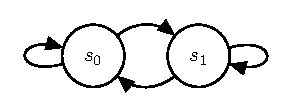
\includegraphics[labelmtd=policyreturn]{img/thesis_plots_mtd.pdf}
    \caption{延迟策略性能的理论洞察示意图。
    x 轴表示给定策略所达到状态分布的抽象量，y 轴表示该策略的性能。
    外层椭圆表示所有随机历史依赖和无延迟策略的集合。
    最优无延迟策略将是该椭圆的最上端点。
    随着延迟 $\delay$ 增加，可达到的回报和状态分布集合收缩，直至延迟变为无穷，此时智能体失去所有控制。}
    \label{fig:evolution_delay}
\end{figure}


\subsection{在 ISM-MDP 中学习}

\glspl{ismmdp} 在通过状态增广被视为 \glspl{mdp} 时，具有特定的结构，本节将研究该结构，以理解哪些文献中的算法可能适用于它们。

首先，一个有问题的结果是 \glspl{ismmdp} 通常不是\emph{单链（unichain）}的，即使底层 \gls{mdp} 是单链的。当任何平稳确定性策略的转移矩阵是单链时，\gls{mdp} 是单链的 \cite[Section~8.3.1]{puterman1994markov}（也见 \Cref{def:unichain_mc}）。在本节中，提及 \glspl{ismmdp} 时，我们指的是按照 \Cref{prop:equ_mdp_is_mtdmdp} 可转化为的 \gls{mdp}。

\begin{prop}
\label{pp:unichain_ismmdp}
    存在这样的 \glspl{ismmdp}，即使底层 \gls{mdp} 是单链的，它们也不是单链的。
\end{prop}
\begin{proof}
    在基于单链 \gls{mdp} 构建的 \gls{ismmdp} 中，考虑确定性平稳策略 $\pi$，给定增广状态 $x=(s,a_1,\dots,a_\delay)$ 时：
    \begin{align*}
        \pi(x) = a_\delay.
    \end{align*}
    则该策略在 $\augmentedstatespace$ 上恰好诱导出 $\cardinal{\actionspace}$ 条链。
\end{proof}


\begin{remark}
    前一个证明中定义的策略访问所有状态 $s\in\statespace$，因为底层 \gls{mdp} 是单链的，且策略 $\pi(s) = a$ 是确定性平稳的。然而，它并不访问 $\augmentedstatespace$ 中的所有增广状态。
\end{remark}

上述结果意味着某些算法，如 UCRL~\cite{auer2006logarithmic}，不能直接应用于具有增广状态的 \glspl{ismmdp}。更有希望的方向是 UCRL2~\cite{auer2008near}，它适用于\emph{连通（communicating）} \glspl{mdp} \cite[Section~8.3.1]{puterman1994markov}（也见 \Cref{def:communicating_mdp}）。

\begin{prop}[连通的 ISM-MDP]
\label{pp:communicating_ismmdp}
    考虑一个连通的 \gls{mdp} $\markovdecisionprocess$ 和建立在其上的 \gls{ismmdp} $\delayedmarkovdecisionprocess_{\boldsymbol\lambda}$。那么该 \gls{ismmdp} 也是连通的。
\end{prop}
\begin{proof}
    首先证明常值延迟 \gls{dmdp} 的结果，再证明推广到 \gls{ismmdp}。

    对于延迟策略 $\delayedpolicy$，记 $(p^\delayedpolicy)^{(k)}(s'\vert x)$ 为从 $x$ 中的状态 $s$ 出发，应用增广状态中最旧的 $k$ 个动作后，环境状态为 $s'$ 的概率。如果 $k>\delaymax$，则后续动作由 $\delayedpolicy$ 采样。类似地，对于无延迟策略 $\pi$，记 $(p^\pi)^{(k)}(s'\vert s)$ 为从 $s$ 出发遵循策略 $\pi$ 执行 $k$ 步后，环境状态为 $s'$ 的概率。

    设 $x=(s,a_1,\dots,a_\delay)$ 和 $x'=(s',a_1',\dots,a_\delay')$ 为 $\delayedmarkovdecisionprocess_{\boldsymbol\lambda}$ 的两个增广状态。设 $s''\in\statespace$ 使得 $(p^\delayedpolicy)^{(\delaymax)}(s''\cdot x)>0$。由于底层 \gls{mdp} 是连通的，存在无延迟策略 $\pi\in\Pi^{\text{SD}}$ 和 $k\in\naturalnumbers$ 使得 $(p^\pi)^{(k)}(s'\vert s'')>0$。设 $k$ 为最小的这样的数。现在记 $\tau$ 为无延迟 \gls{mdp} 中的一条轨迹，它先从 $s$ 到 $s''$（$\delaymax$ 步），然后从 $s''$ 到 $s'$（$k$ 步），且概率 $p^\pi(\tau)>0$。上述性质保证这样的轨迹存在。具体地，记
    \begin{align*}
        \tau=(s,a_0^\star,s_1^\star,a_1^\star,\dots,a_{\delaymax-1}^\star,s'',a_{\delaymax}^\star,\dots,s_{k+\delaymax-1}^\star,a_{k+\delaymax-1}^\star,s').
    \end{align*}
    可以将 $s$ 重写为 $s_0^\star$，$s''$ 重写为 $s_{\delaymax}^\star$；对于 $x'$ 中包含的动作，记 $a_i'$ 为 $a_{k+\delaymax+i-1}^\star$。现在准备定义一个候选的平稳确定性延迟策略 $\delayedpolicy$，以非零概率将我们从 $s$ 带到 $s'$。定义 $x_i^\star=(s_i^\star,a_i^\star,\dots,a_{i+\delaymax-1}^\star)$，策略定义如下：
    \begin{align*}
        &\delayedpolicy(x_i^\star) = a_{i+\delaymax}^\star.
    \end{align*}
    其他增广状态的定义无关紧要，可以自由指定。
    该策略有非零概率从 $x$ 到达 $x'$，但不清楚它是否真正定义了一个策略。
    实际上，智能体可能两次面对相同的增广状态，而上述策略会指示两个不同的动作。换句话说，$\delayedpolicy$ 可能不是正确定义的函数。下面证明这不是问题，或者当它发生时，可以应用简单的修改。

    设 $i,j\in\naturalnumbers$ 使得 $\delaymax<i<j$ 且 $x_i^\star=x_j^\star$，但 $\delayedpolicy(x_i^\star)\neq \delayedpolicy(x_j^\star)$。则从 $s_j^\star$ 到 $s$ 的轨迹长度为 $\delaymax+k-j<\delaymax+k-i$，但 $s_j^\star=s_i^\star$，因此时刻 $j$ 之后定义的无延迟策略可以在时刻 $i$ 应用，以严格正概率产生更短的轨迹。这与 $\tau$ 的假设矛盾。还有一个小的复杂性；正如读者注意到的，我们假设了 $\delaymax<i<j$。确实，由于我们无法控制前 $\delaymax$ 个动作，在第 $\delaymax$ 步之后出现的增广状态可能已经在最初的 $\delaymax$ 步中出现过。然而，这相当于智能体已经处于轨迹 $\tau$ 的更高级部分，因此可以将较高索引对应的增广状态的动作保留为 $\delayedpolicy$ 的值。这确保了 $\delayedpolicy$ 是正确定义的平稳确定性策略，且满足 $(p^\delayedpolicy)^{(\delaymax+k)}(x'\vert x)>0$。因此 \gls{dmdp} 是连通的。

    \gls{ismmdp} 的结果如下获得。
    在任何步骤中，$\delaymax$ 位置上的动作被执行的概率非零；因此，整个过程如同 $\delaymax$-常值延迟 \gls{dmdp} 那样采样轨迹的概率非零。根据上述结论，由于后者是连通的，因此在原始 \gls{ismmdp} 中从 $x$ 出发到达 $x'$ 的概率非零。
\end{proof}

\begin{remark}
    如证明所示，且因为 \glspl{ismmdp} 将常值延迟 \glspl{dmdp} 作为特例包含，该结果也表明：若底层 \gls{mdp} 是连通的，则常值延迟 \gls{dmdp} 也是连通的。
\end{remark}

有了这一性质，就可以应用 UCRL2~\cite{auer2008near} 在 \gls{ismmdp} 中学习策略。如 \Cref{subsec:theoretical_rl} 所述，UCRL2 的遗憾依赖于 \gls{mdp} 直径的概念，定义见 \Cref{def:diameter}。\gls{ismmdp} 中的直径显然以底层 \gls{mdp} 的直径为下界。通过将 \cite{auer2008near} 的结果应用于这一特殊情况，可以给出直径的更好下界。

\begin{prop}
    设 $\delayedmarkovdecisionprocess_{\boldsymbol\lambda}$ 为最大延迟为 $\delaymax$ 的 \gls{ismmdp}，且其动作空间包含两个或以上动作，则
    \begin{align*}
        D(\delayedmarkovdecisionprocess_{\boldsymbol\lambda})\geq \delaymax-3 + \log_{\cardinal{\actionspace}}\cardinal{\statespace}
    \end{align*}
\end{prop}
\begin{proof}
    从 \cite[Corollary~15]{auer2008near} 可知，对于状态空间为 $\statespace$、动作空间为 $\actionspace$ 的某个 \gls{mdp} $\markovdecisionprocess$，
    \begin{align*}
        D(\markovdecisionprocess)\ge\log_{\cardinal{\actionspace}}\cardinal{\statespace}-3.
    \end{align*}
    将此结果应用于从 \gls{ismmdp} 获得的状态空间为 $\statespace\times\actionspace^{\delaymax}$ 的增广 \gls{mdp}，即完成证明。
\end{proof}

这里看到延迟对直径的加性影响。注意，即使项 $-3 + \log_{\cardinal{\actionspace}}\cardinal{\statespace}$ 可能为负，直径也永远不会小于 $\delaymax$。为证明这一点，只需考虑两个增广状态其动作不匹配的情况，显然需要超过 $\delaymax$ 个动作才能从一个到达另一个。